\documentclass[]{article}
\usepackage[margin=0.9in]{geometry}

\usepackage{enumitem}
\usepackage{graphicx}
\usepackage{hyperref}
\usepackage{float}
\usepackage{fancyvrb,newverbs,xcolor}
\usepackage{hyperref}

\usepackage{listings}
\lstset{
	language=bash,
	basicstyle=\ttfamily
}

\providecommand{\tightlist}{%
	\setlength{\itemsep}{0pt}\setlength{\parskip}{0pt}}


% Back tick style from gfm
\definecolor{Light}{gray}{.90}

\let\oldtexttt\texttt
\renewcommand{\texttt}[1]{
	\colorbox{Light}{\oldtexttt{#1}}
}

\graphicspath{{images/user-manual/}{images/logo/}}

\hypersetup{
	colorlinks=true,
	linkcolor=blue,
	filecolor=magenta,
	urlcolor=cyan,
}

%opening
\title{
	\vspace{-1.5cm}
	
\includegraphics[scale=0.7]{docks_round_512.png}
	\\[1cm]
	User Manual for Docks}
	\author{\textbf{Team}: TripleParity\\
	\textbf{Client}: Compiax\\
	\\
	\textbf{Team Members}\\
	Francois Mentz\\
	Connor Armand du Plooy\\
	Raymond De Vos\\
	Evert Geldenhuys\\
	Anna-Marié Helberg\\
	Paul Wood
}
\date{}

\begin{document}

\maketitle

\tableofcontents

\pagebreak

\section{System Overview}
% TODO(egeldenhuys): How much of Docker will we explain?

This document assumes knowledge of how Docker works. For more information
read:
\begin{itemize}
	\tightlist
	\item \href{https://docs.docker.com/engine/}{About Docker Engine}
	\item \href{https://docs.docker.com/engine/docker-overview/}{Docker Overview}
	\item \href{https://docs.docker.com/engine/swarm/key-concepts/}{Swarm Mode Key Concepts}
\end{itemize}

Docks provides a web interface for managing a Docker Swarm.
Along with an easy to use interface Docks provides security by only
allowing registered users to manage Docker. Docks exposes the same
functionality as the Docker Command Line Interface.

% TODO(egeldenhuys): Guest users
Docks allows developers and system administrators to manage the
deployment of applications without requiring SSH access to a server.


\section{System Configuration}
Docks consists of two subsystems:
\begin{itemize}
	\item Docks Web Interface
	\item Docks API Server
\end{itemize}

The web interface can be served from any static file server such as GitHub pages
and will communicate with the Docks API server through the web browser.

The Docks API server is deployed on a Manager Node in the Docker Swarm

\begin{figure}[h!]
	\centering
	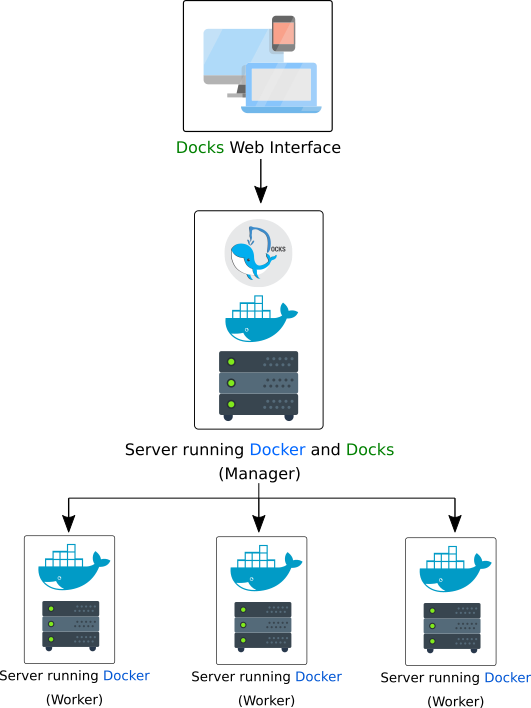
\includegraphics[scale=0.6]{deployment_diagram.png}
	\caption{Docks Deployment Diagram}
\end{figure}

\pagebreak

\section{Installation}
% This section was generated by Pandoc from the README.md
% $ sudo dnf install pandoc
% $ pandoc -s README.md -o README.tex
% Copy Getting Started section to this document
% Fix links or anything that was not successfully converted to latex

\begin{enumerate}
	\def\labelenumi{\arabic{enumi}.}
	\tightlist
	\item
	  Install \href{https://docs.docker.com/install/}{Docker} 17.06.2-ce or higher
	\item
	  Install \href{https://docs.docker.com/compose/install/}{Docker Compose}
	\item
	  Create a Swarm using \texttt{sudo\ docker\ swarm\ init}
	\item
	  Clone \texttt{https://github.com/TripleParity/docks.git}
	\item
	  Run \texttt{sudo\ docker-compose\ pull} to download the required
	  images
	\item
	  Run
	  \texttt{sudo\ docker\ stack\ deploy\ -c\ docker-compose.yml\ docks} to
	  deploy Docks
	\item
	  Run
	  \texttt{sudo\ docker\ stack\ deploy\ -c\ docker-compose-nginx.yml\ demo}
	  to deploy a sample application
	\item
	  Browse to \url{http://127.0.0.1:4200} to view the Docks web interface
	\item
	  To remove Docks from the system run the following commands:
	
	  \begin{itemize}
	  \tightlist
	  \item
		\texttt{sudo\ docker\ stack\ rm\ docks}
	  \item
		\texttt{sudo\ docker\ stack\ rm\ demo}
	  \end{itemize}
	\end{enumerate}

\subsection{Configuration}
% I am not sure where this section should go

\subsubsection{Docks Web Interface}
The following parameters can be configured in the \texttt{docker-compose.yml} file

% NOTE: cannot use _ in \texttt: escape it
\begin{itemize}
	\tightlist
	\item \texttt{DOCKS\_API\_ADDRESS} - The address of the Docks API server
	\item \texttt{ports} - The ports to listen on
\end{itemize}

\subsubsection{Docks API}
The following parameters can be configured in the \texttt{docker-compose.yml} file

\begin{itemize}
	\tightlist
	\item \texttt{JWT\_SECRET} - The secret key used during authentication requests
	\item \texttt{DOCKS\_DB\_ADDRESS} - The address of the database
	\item \texttt{POSTGRES\_PASSWORD} - The password for the \texttt{postgres} database user
	\item \texttt{ports} - The ports to listen on
\end{itemize}

\section{Getting Started}
The web interface will be available at \url{http://127.0.0.1:4200} after following the Installation instructions.
The database will automatically be initialized and the default user will
be created:
\begin{itemize}
	\tightlist
	\item Username: \texttt{admin}
	\item Password: \texttt{admin}
\end{itemize}

\begin{figure}[h!]
	\centering
	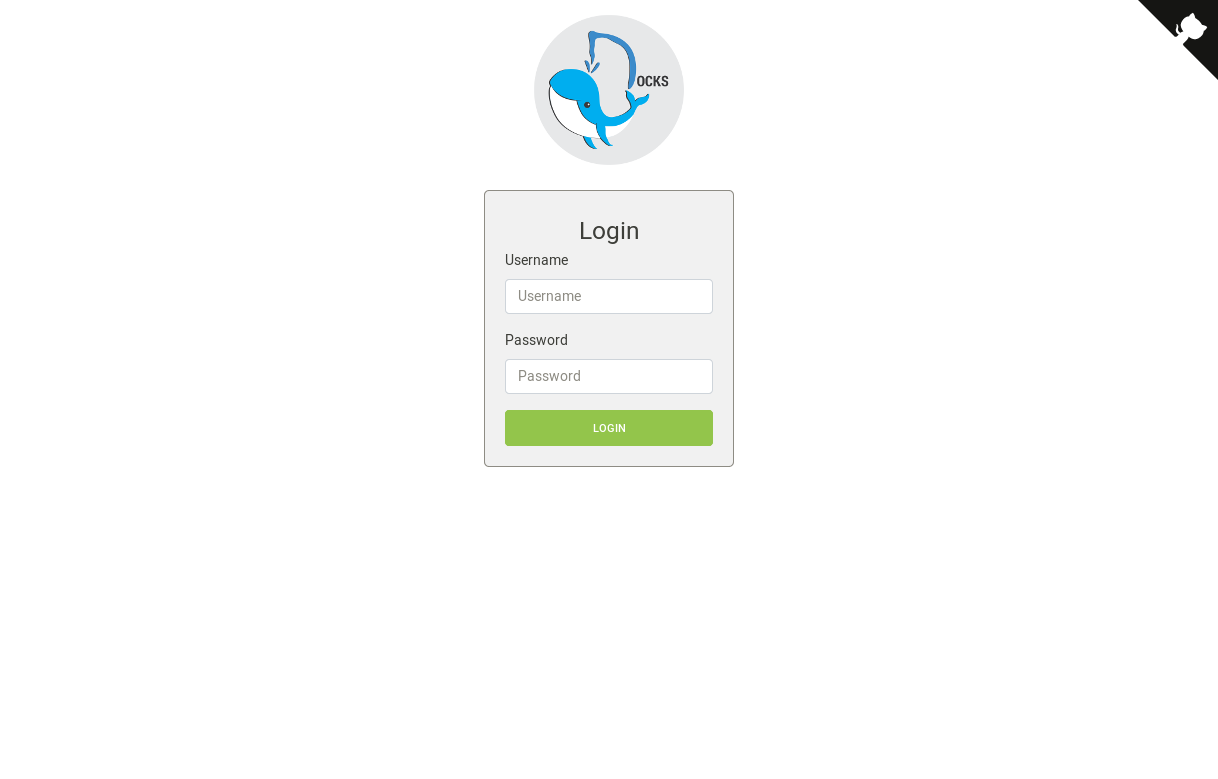
\includegraphics[scale=0.4]{login.png}
	\caption{Login Page}
\end{figure}

It is strongly recommended to change the password as soon as possible.
This will be explained further in \nameref{sec:user_management}

\begin{figure}[H]
	\centering
	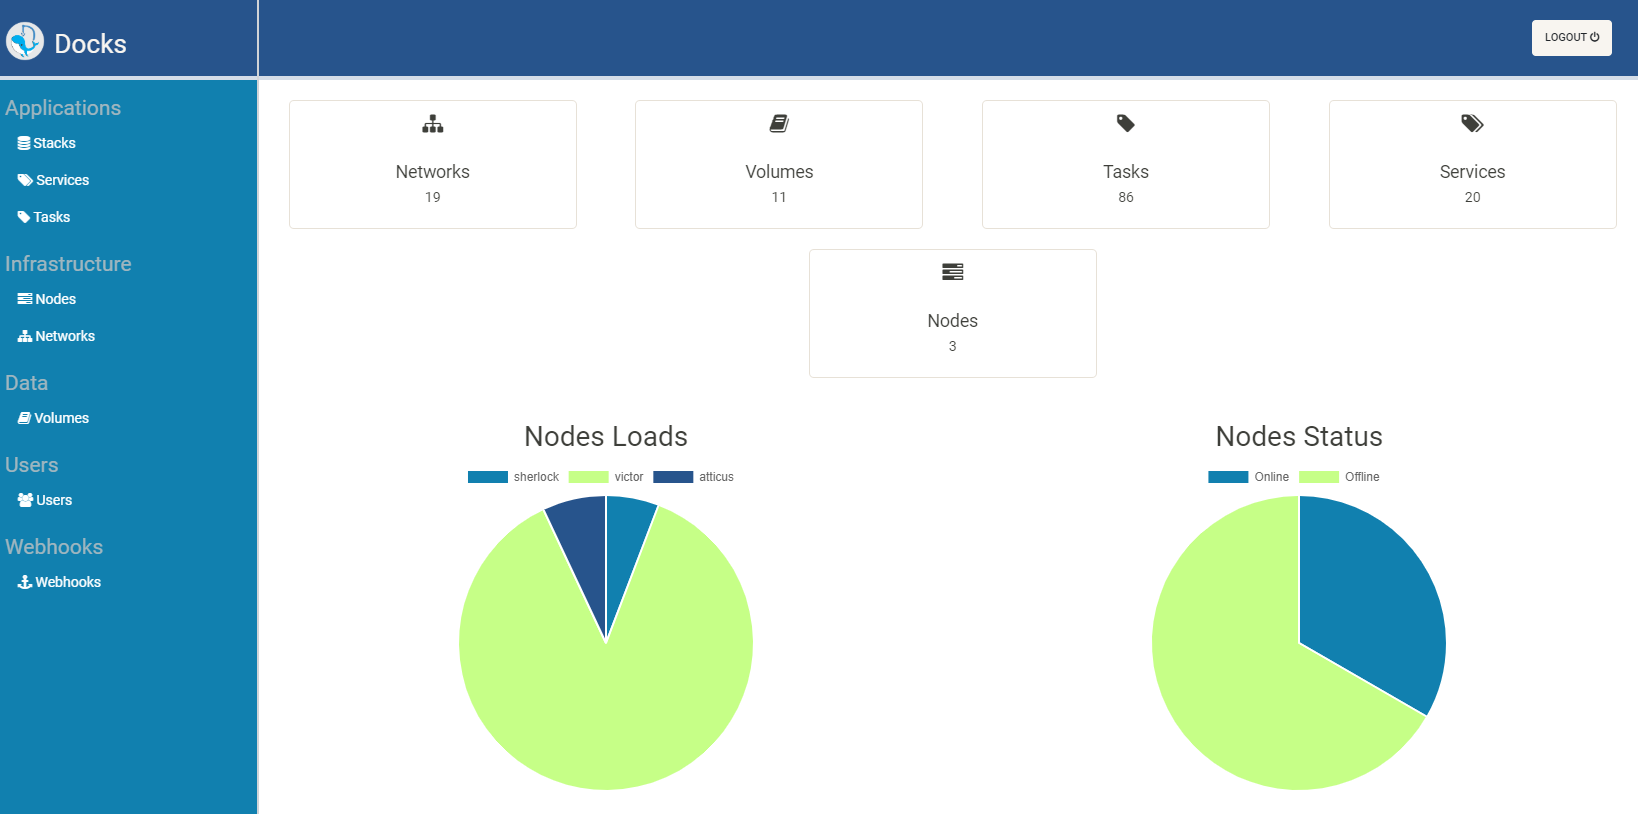
\includegraphics[scale=0.4]{home.png}
	\caption{Home Screen}
\end{figure}

\section{Using the System}


\subsection{Tasks}
A service consists of Tasks. Tasks can only be viewed - they are managed by Docker
as part of services.

\subsubsection{Viewing Tasks}
The table displays the following information:
\begin{itemize}
	\tightlist
	\item Name of the task
	\item Image that the task is running
	\item State of the task.
	Green means the task is running, 
	red indicating it has stopped and blue indicating it is preparing
	\item Node ID on which the task is running
\end{itemize}

\begin{figure}[H]
	\centering
	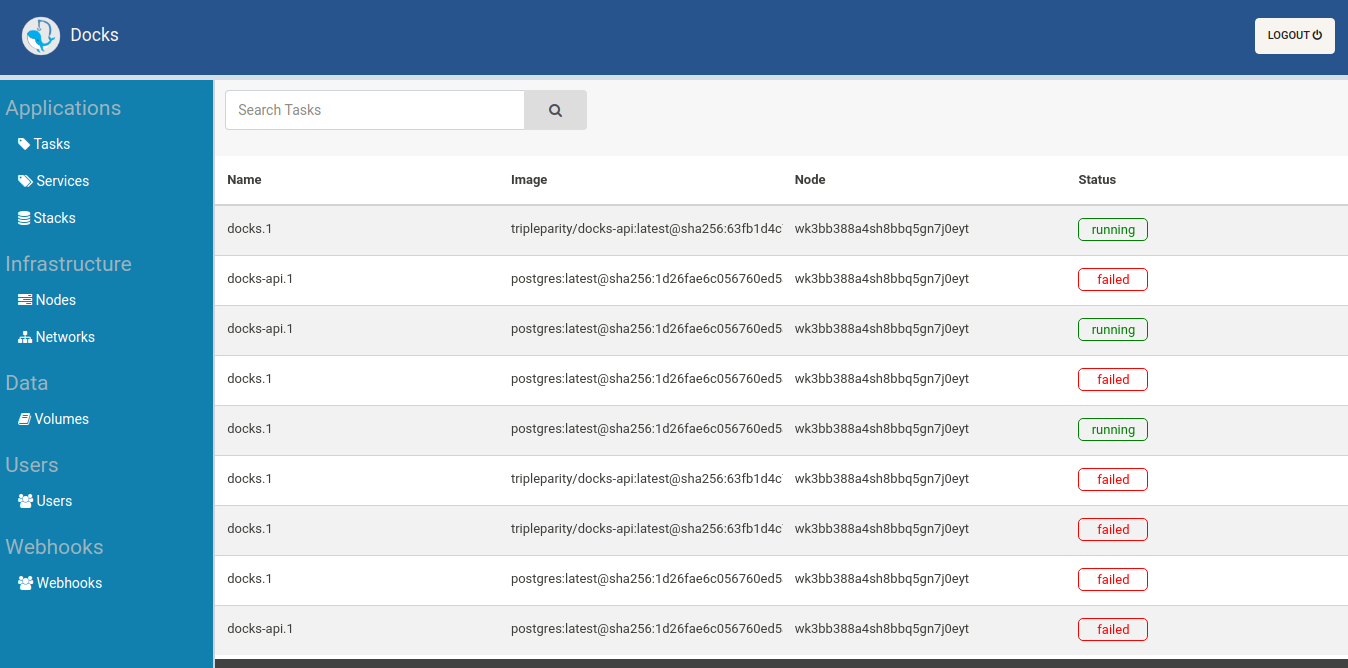
\includegraphics[scale=0.4]{tasks.png}
	\caption{Task View}
\end{figure}

\subsubsection{Viewing Task Details}
From the task view, a task can be clicked to open up an new page
on which details of that specific task is displayed.

\begin{figure}[H]
	\centering
	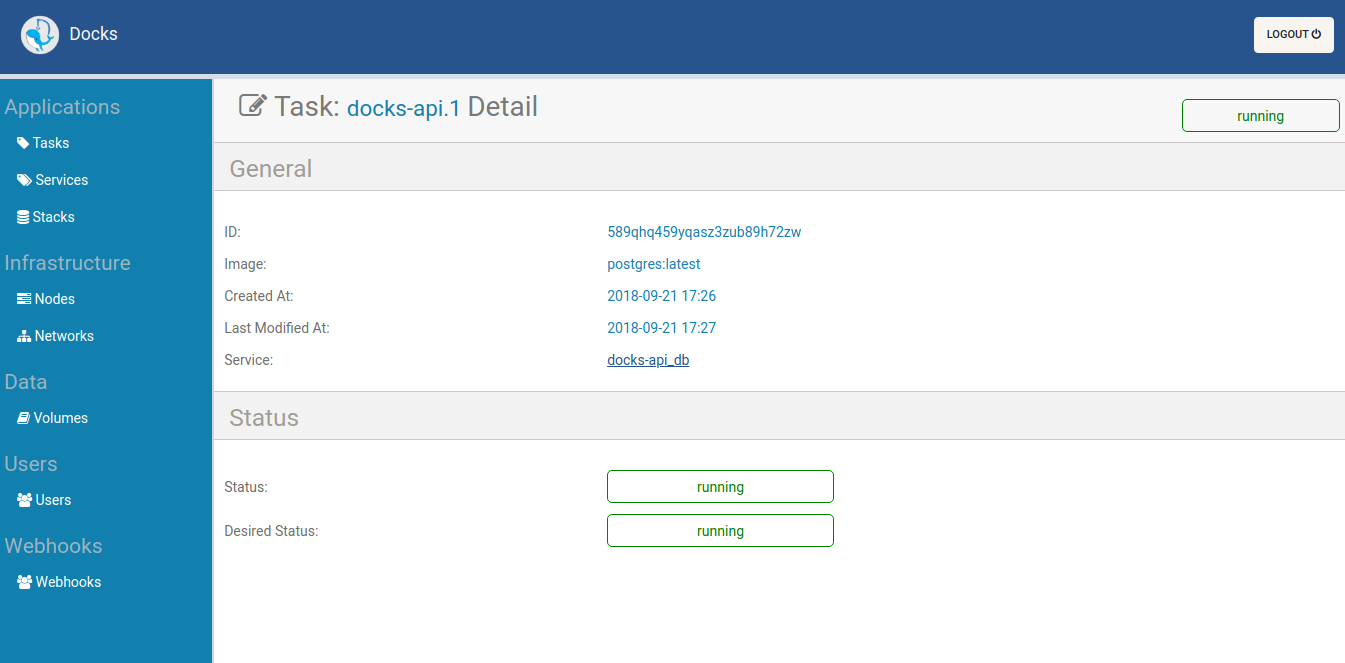
\includegraphics[scale=0.4]{task_details.png}
	\caption{Task Detail View}
\end{figure}

\subsection{Services}
A stack consists of services. The service list view provides a sortable 
and searchable table for deployed services.

\subsubsection{Viewing Services}
The table displays the following information:
\begin{itemize}
	\tightlist
	\item Name of the service
	\item Image that the service is running
	\item Mode of the service
	\item Replicas of that services running
	\item Port of which the service is listening
\end{itemize}

\begin{figure}[H]
	\centering
	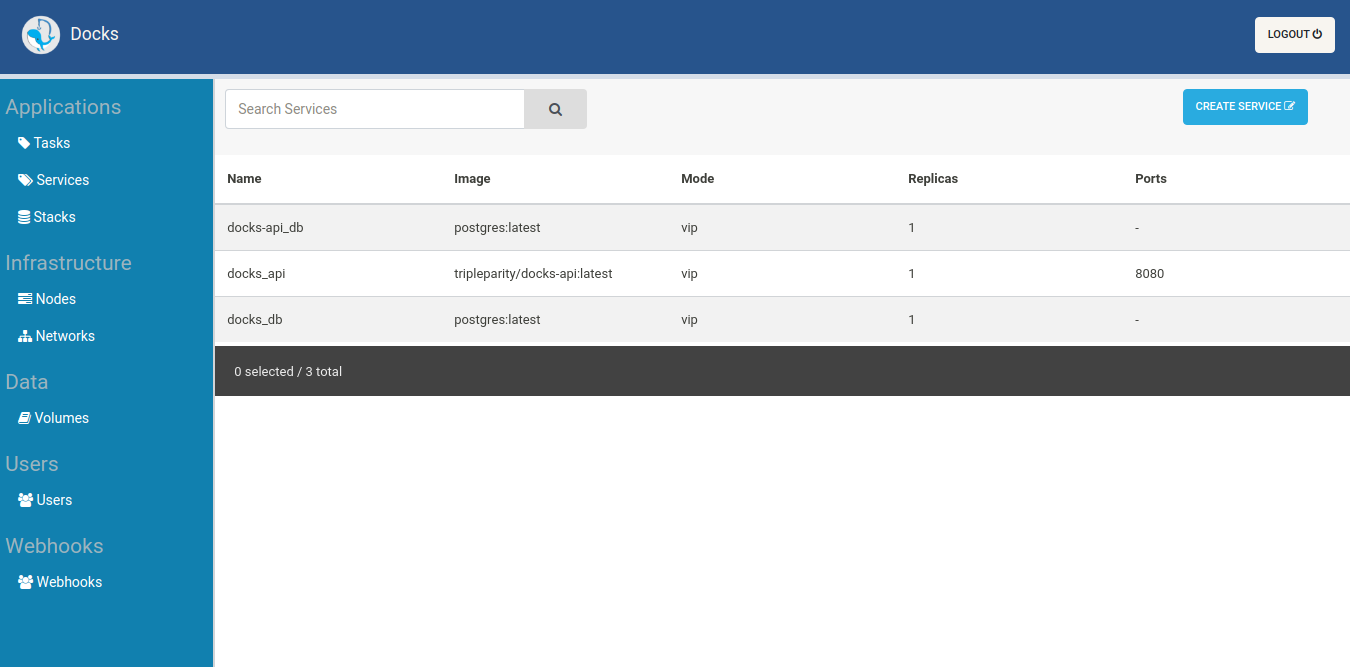
\includegraphics[scale=0.4]{services.png}
	\caption{Service View}
\end{figure}


\subsubsection{Viewing Service Details}
From the service view, a service can be clicked to open up an new page
on which details of that specific service are displayed.

\begin{figure}[H]
	\centering
	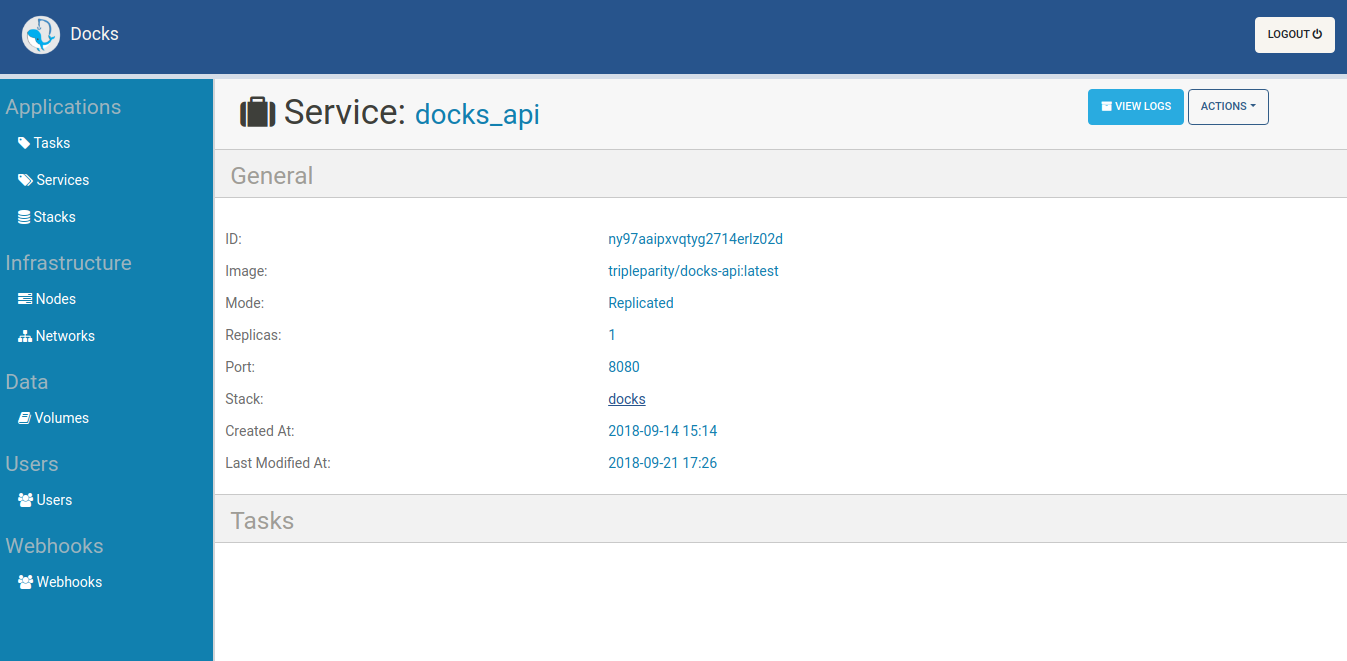
\includegraphics[scale=0.4]{service_details.png}
	\caption{Service Detail View}
\end{figure}

\subsubsection{Viewing Service Logs}
From the service detail view, the logs page can be opened to view the 
complete log for that service.

\begin{figure}[H]
	\centering
	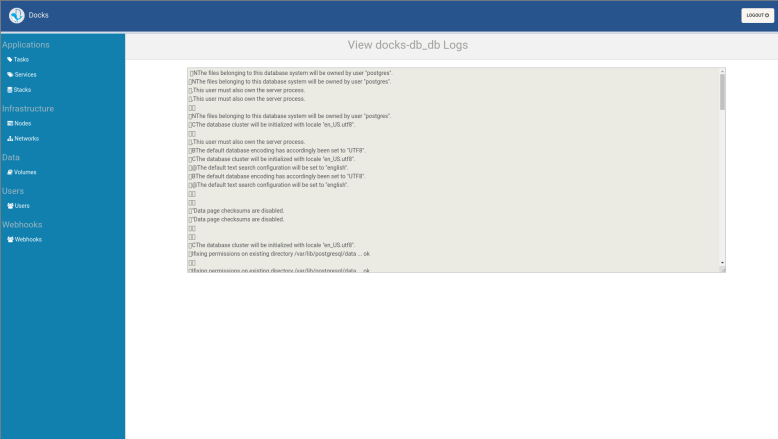
\includegraphics[scale=0.4]{services_logs.png}
	\caption{Service Log View}
\end{figure}

\subsection{Stacks}
The concept of a Stack is the core feature of Docker.
A Stack describes Services (applications) and how they should be deployed.

\subsubsection{Viewing Stack}
The table displays the following information:
\begin{itemize}
	\tightlist
	\item Name of the stack
	\item Number of services that belongs to the stack 
\end{itemize}

\begin{figure}[H]
	\centering
	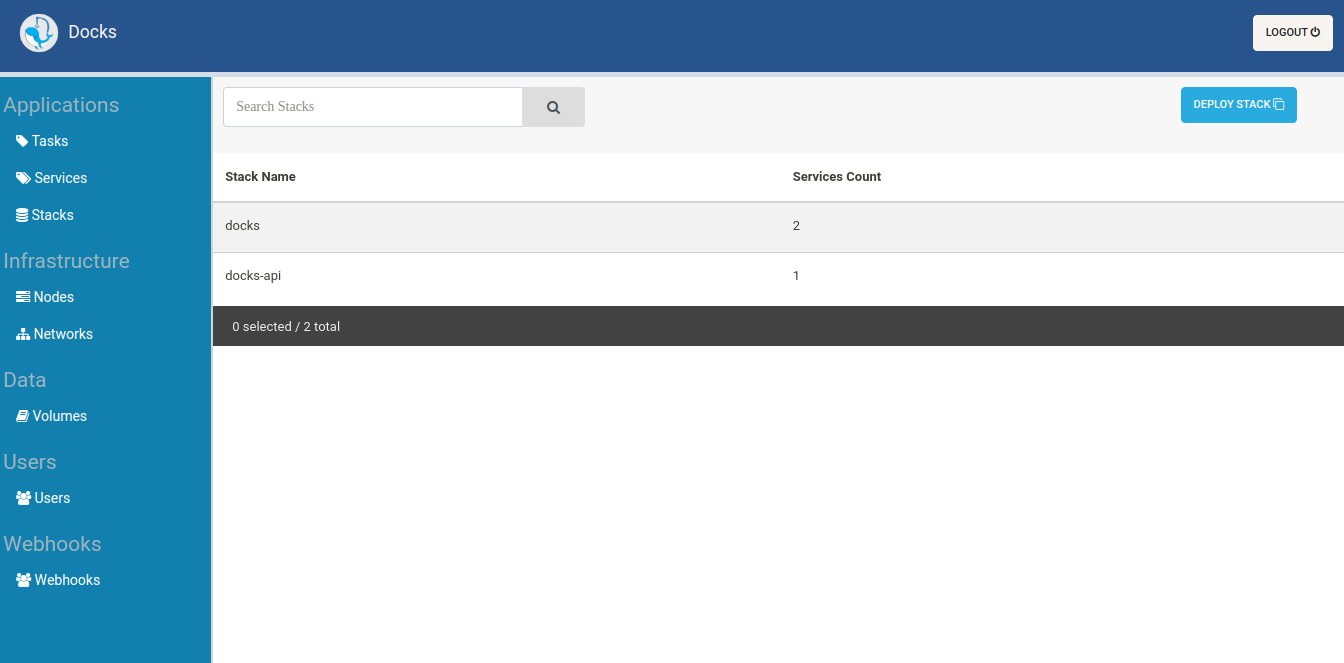
\includegraphics[scale=0.4]{stacks.png}
	\caption{List of Stacks in the Swarm}
\end{figure}

\subsubsection{Deploying a Stack}
Docks allows the user to deploy their own Stack (Application) by uploading
a Stack file. Pre-configured stacks can also be selected for deployment,
such as Wordpress, Nginx, and MongoDB. The Stack File should be modified
to fit the needs of the administrator and the system.

The Stack should be given a unique name to identify it in the system.

\begin{figure}[H]
	\centering
	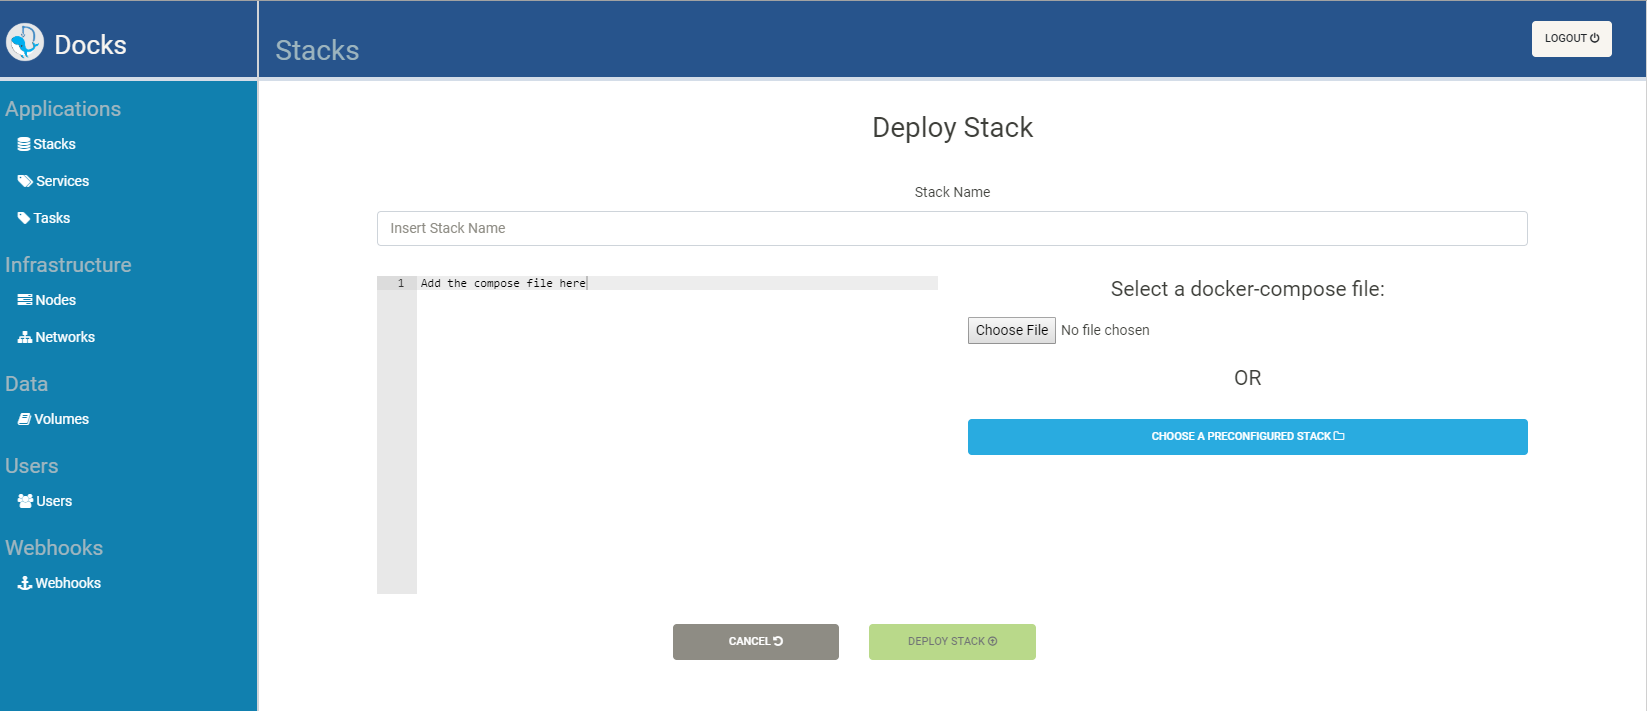
\includegraphics[scale=0.4]{stacks_deploy.png}
	\caption{Deploying a Stack}
\end{figure}

\subsubsection{Updating a Stack}
\label{sec:stacks_update}

By uploading a modified Stack file Docker will automatically update the deployed
Stack to match the Stack file.

Reasons for updating the stack may include:
\begin{itemize}
	\item Updating to a new version
	\item Adding a new application to the Stack
	\item Changing the port for a running application
	\item Attaching new volumes to applications for extra storage
	\item Changing environmental variables used for configuration
\end{itemize}

\begin{figure}[H]
	\centering
	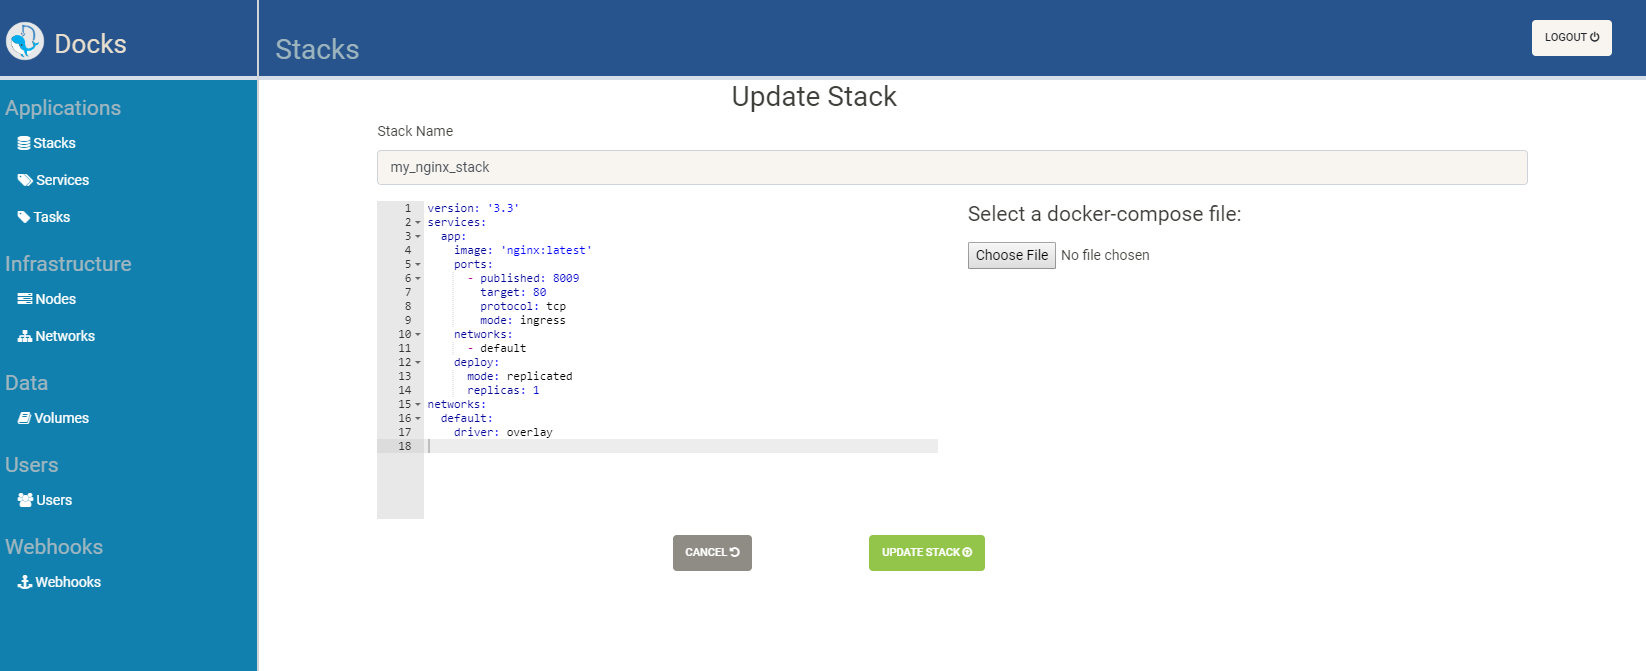
\includegraphics[scale=0.4]{stacks_edit.png}
	\caption{Updating a Stack}
\end{figure}

\subsection{Node Management}
Docker swarm is a concept that clusters single, separate docker hosts into a single
virtual docker host. It consists of manager nodes that delegate jobs and load balance between
worker nodes.

\subsubsection{Viewing Nodes}
The table displays the following information:
\begin{itemize}
	\tightlist
	\item Name of the nodes
	\item Engine version of the node
	\item IP Address of the node
	\item Availability of the node 
	Green means the nodes is active, 
	red indicating it has stopped and blue indicating it is preparing
	\item Role of the node
	\item State of the node 
	Green means the nodes is active, 
	red indicating it has stopped and blue indicating it is preparing
	\item Number of CPU's assigned to the node
	\item Memory assigned to the node
\end{itemize}

\begin{figure}[H]
	\centering
	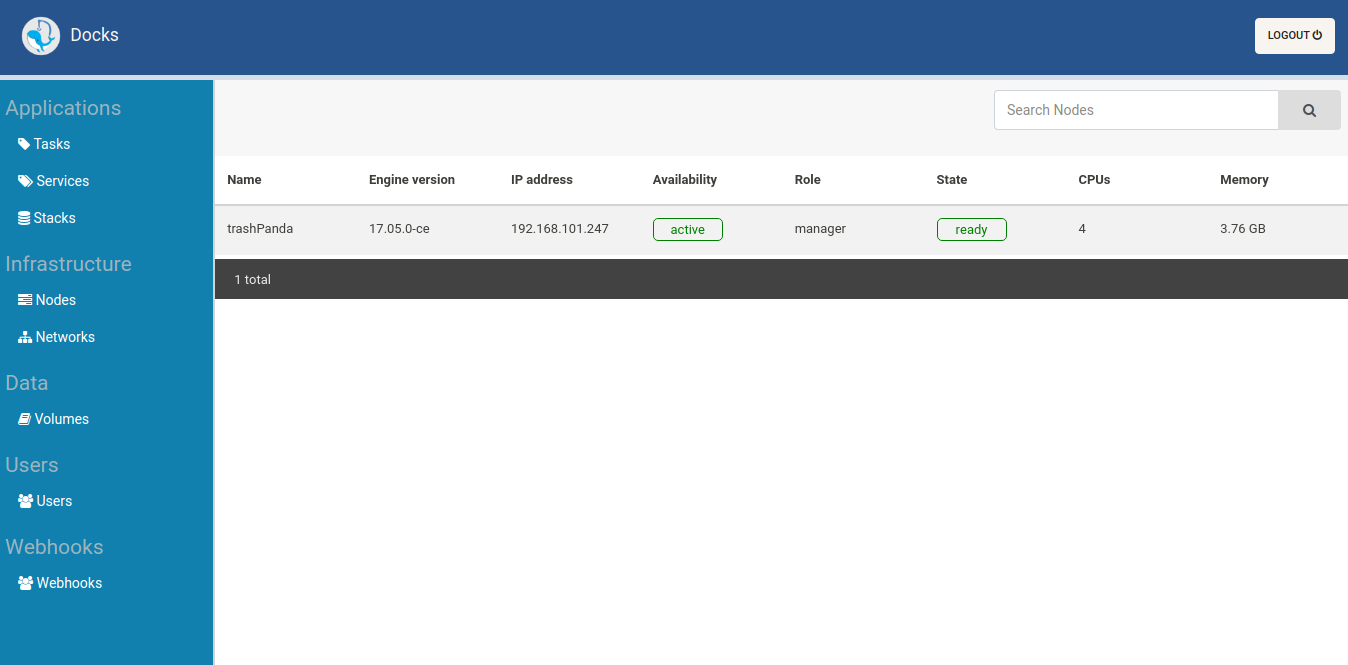
\includegraphics[scale=0.4]{nodes.png}
	\caption{Nodes View}
\end{figure}

\subsection{Network Management}
Docker networks allow a user to connect containers with services or
containers and services to non-Docker workloads.

\subsubsection{Viewing Networks}
The table displays the following information:
\begin{itemize}
	\tightlist
	\item Name of the network
	\item Driver assigned to the network
\end{itemize}

\begin{figure}[H]
	\centering
	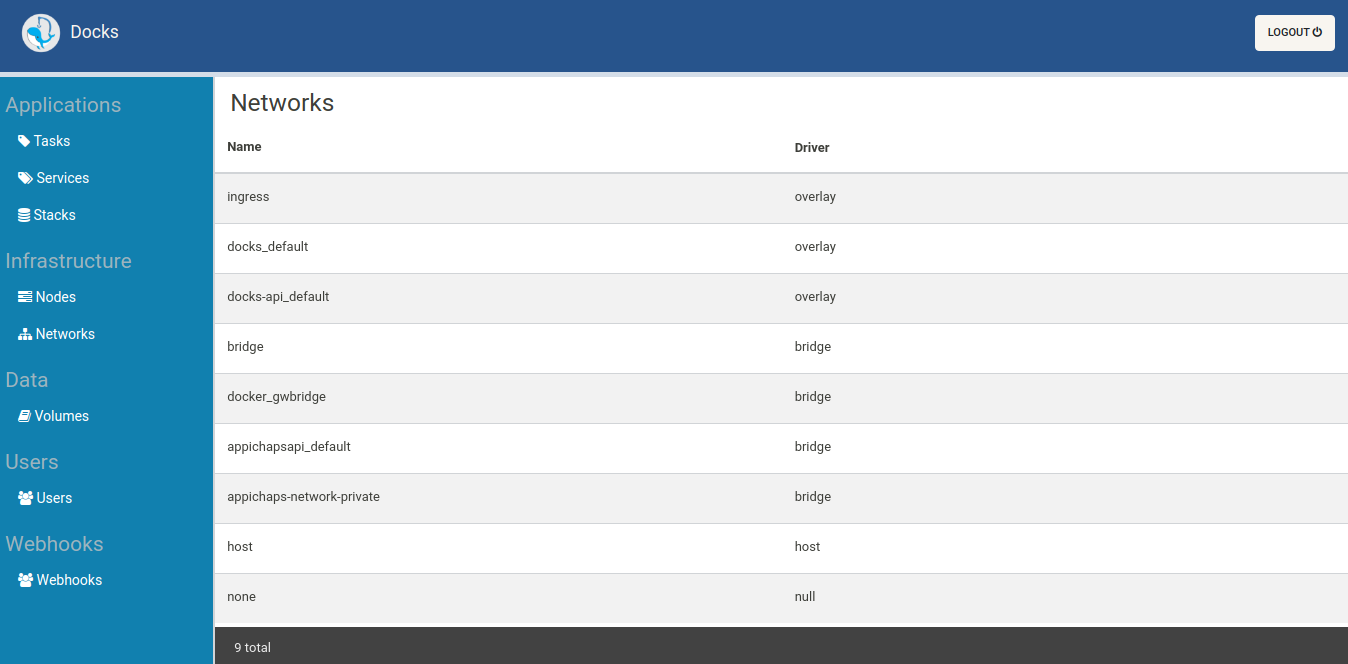
\includegraphics[scale=0.4]{networks.png}
	\caption{Networks View}
\end{figure}


\subsection{Volume Management}
Volumes are used with persistent data generated and used by Docker containers.

\subsubsection{Viewing Volumes}
The table displays the following information:
\begin{itemize}
	\tightlist
	\item Name of the volume
	\item Driver assigned to volume
\end{itemize}

\begin{figure}[H]
	\centering
	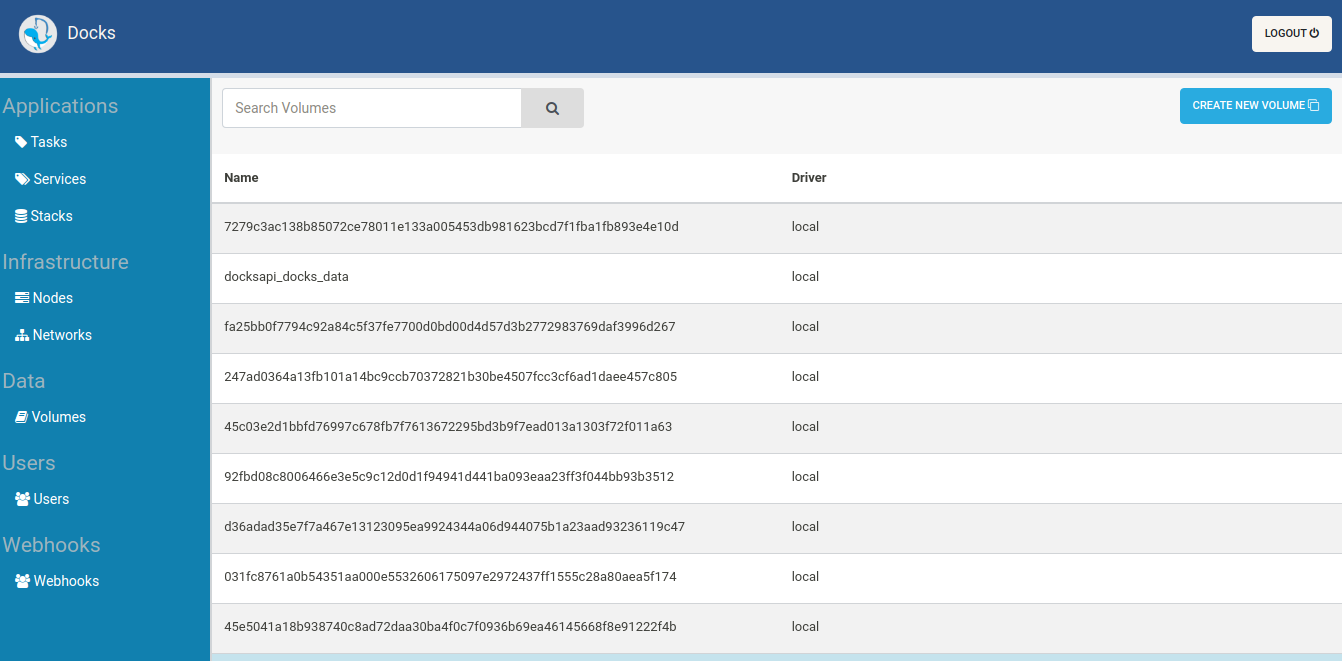
\includegraphics[scale=0.4]{volumes.png}
	\caption{Volumes View}
\end{figure}

\subsubsection{Creating Volumes}
Docks allows the user to create their own volumes. 
The Volums should be given a unique name and assigned to a driver.

\begin{figure}[H]
	\centering
	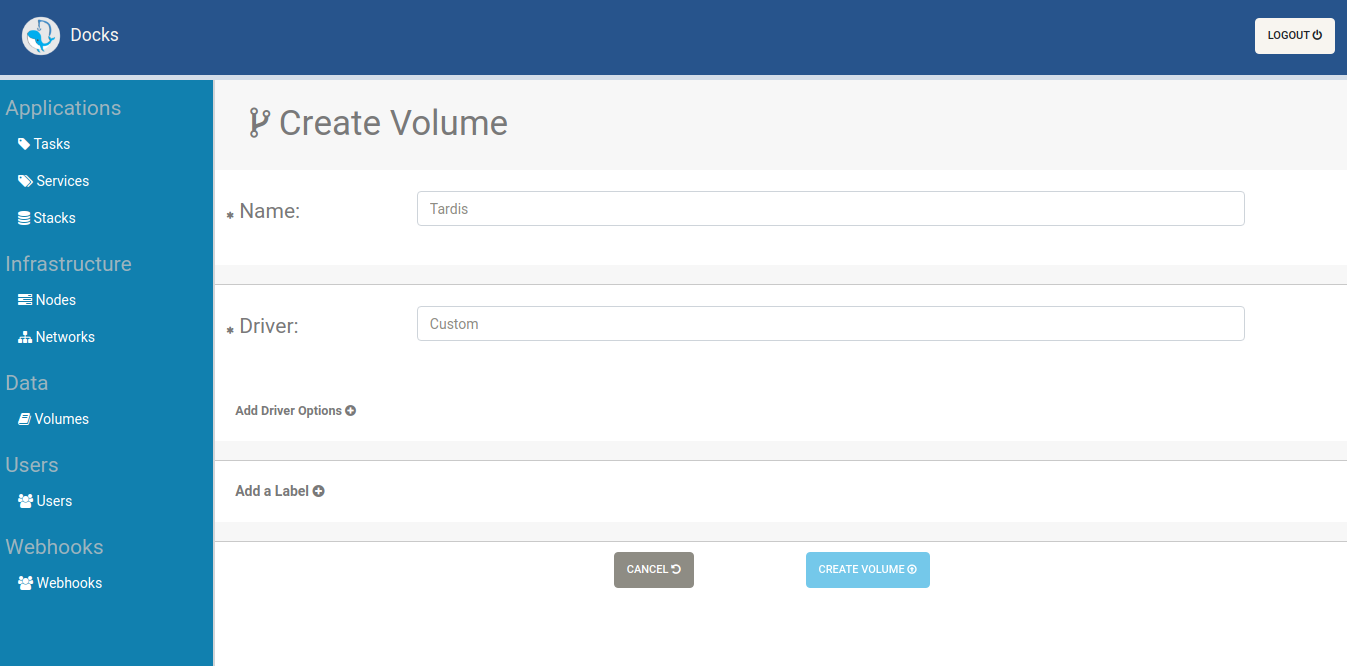
\includegraphics[scale=0.4]{volumes_create.png}
	\caption{Deploying a Stack}
\end{figure}

\subsection{User Management}
\label{sec:user_management}
\subsubsection{Viewing Users}
Only registered users can use Docks. An admin user can create more admin users.
Currently there exists only admin users, so be sure to trust the person that will
be using the account.
\begin{figure}[H]
	\centering
	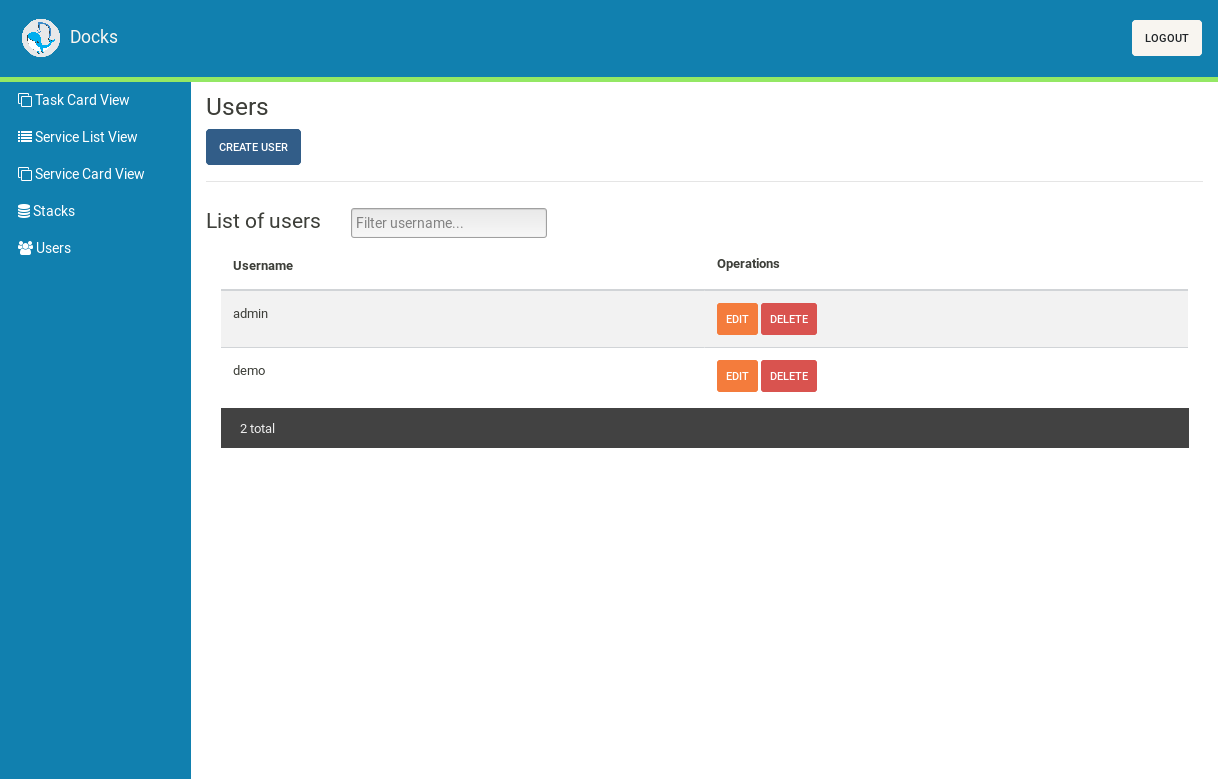
\includegraphics[scale=0.4]{users.png}
	\caption{Users}
\end{figure}

\subsubsection{Creating Users}
Users can be created.

\begin{figure}[H]
	\centering
	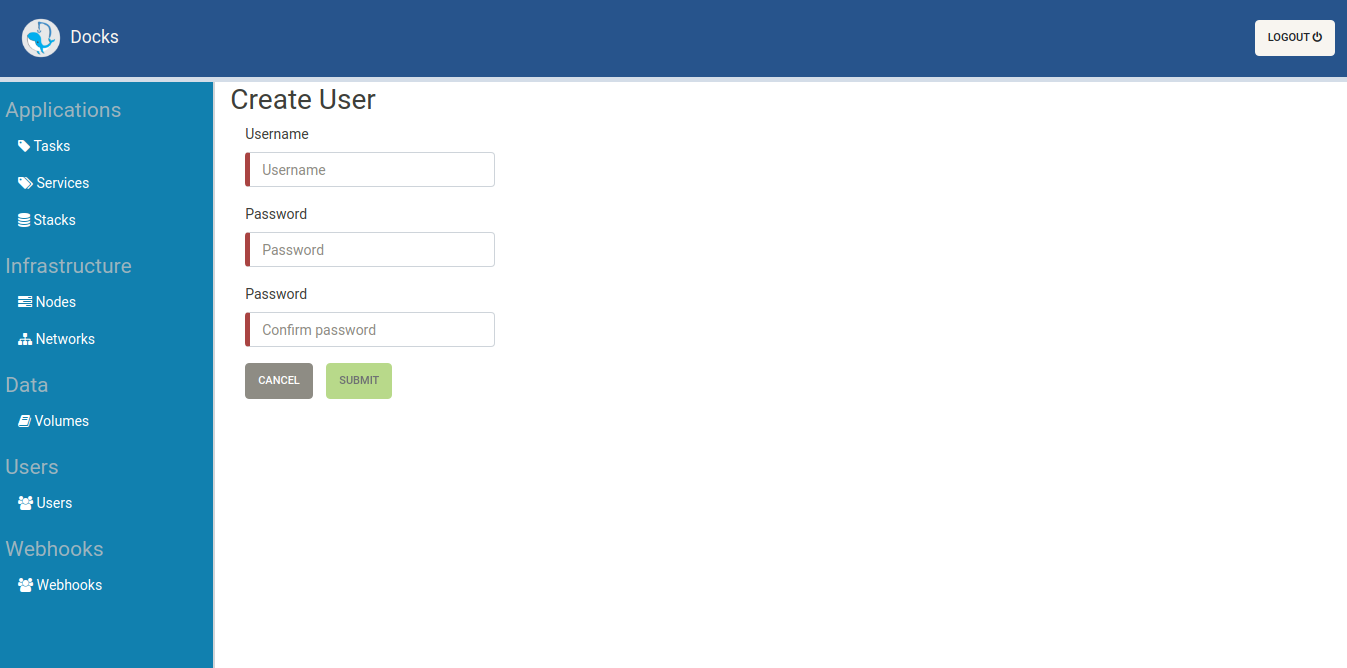
\includegraphics[scale=0.4]{users_create.png}
	\caption{Users}
\end{figure}

\subsubsection{Editing Users}
Passwords can be changed using the Change Password page (Users -> Edit)

\begin{figure}[H]
	\centering
	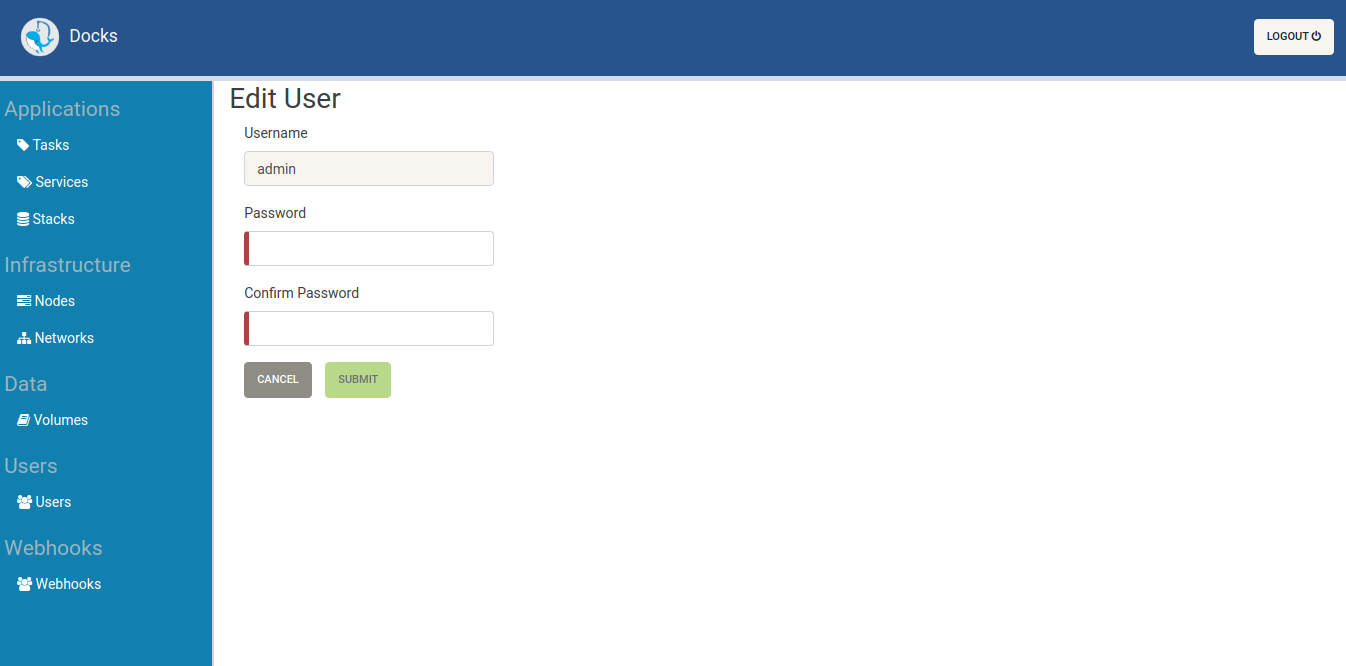
\includegraphics[scale=0.4]{users_edit.png}
	\caption{Users}
\end{figure}

\subsection{Webhooks Management}
Webhooks make it easy for our application to communicate 
flexibly with external services (such as slack). This allows us to 
generate slack notifications

\subsubsection{Creating Webhooks}
This pages allows you create webhooks.

\begin{figure}[H]
	\centering
	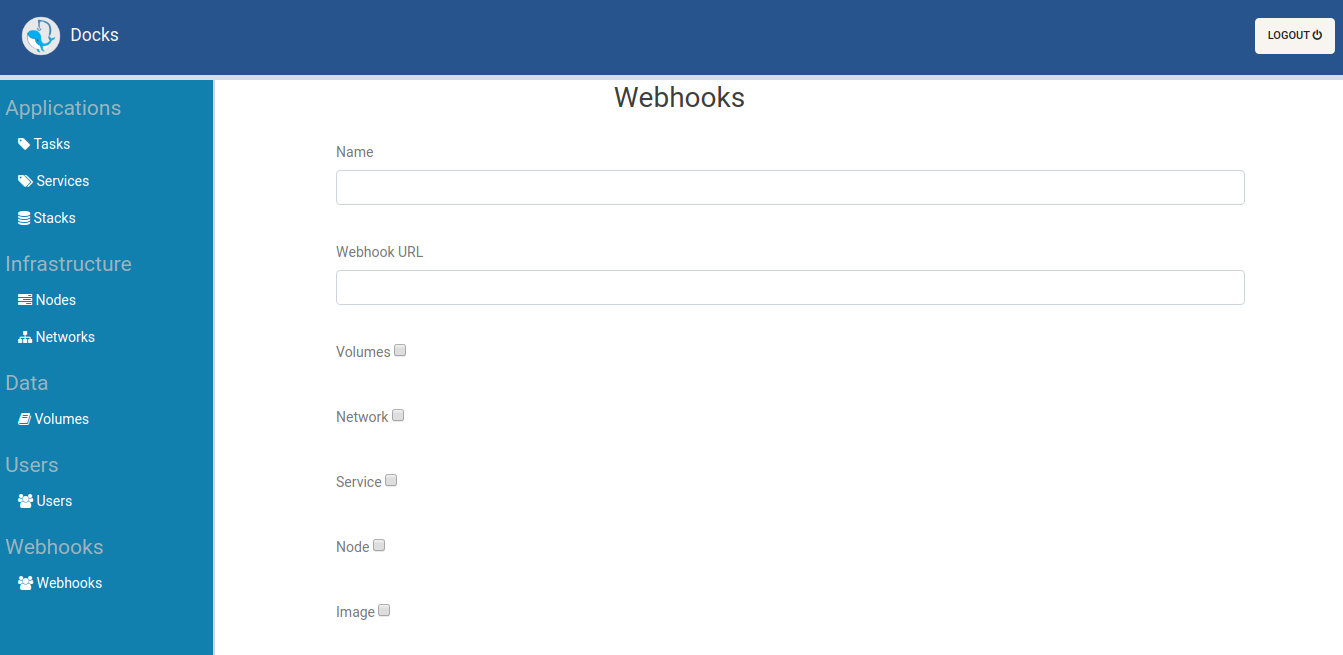
\includegraphics[scale=0.4]{webhooks.png}
	\caption{Webhooks Creation}
\end{figure}

\section{Updating Docks}
Once Docks is deployed, it can be updated as described in \nameref{sec:stacks_update}

Alternatively the respective Stack file can be modified locally as deployed using
\texttt{sudo docker stack deploy -c docker-compose.yml docks}

\section{Troubleshooting}
\subsection{Error: bind: address already in use}
Another service is most likely running on port \texttt{4200}, \texttt{8080} or \texttt{8081}.
The ports for Docks and nginx-demo can be specified in the \emph{docker-compose.yml} 
and \emph{docker-compose-yml} files.

For example to run on port 9000 instead of 4200 make the following changes:

\begin{lstlisting}
    ports:
      - 4200:80
\end{lstlisting}
to
\begin{lstlisting}
    ports:
      - 9000:80
\end{lstlisting}


\end{document}
